\chapter{ACL}
\section{ACL Operation Overview}
An ACL contains a sequential list of permit or deny statements, known as access control entrie (ACEs). ACEs are also commonly called ACL statements. 
\subsection{ACEs Logic Operations}
ACLs are processed in a top down manner. When an ACL is inspected, if the information in a packet header and an ACL statement match, the remaining statements are not examined, and the packet is either denied or permitted through as specified by the ACL. If a packet header does not match an ACL statement, the packet is tested against the next statement in the list. This matching process continues until the end of the list is reached. If no conditions match, the address is rejected.\par 
In a nut shell, ACL always stops testing conditions after the first match, therefore, the order of the ACEs is critical.\par 
At the end of every ACL is a statement is an implicit deny any statement and because of this
statement, an ACL should have at least one permit statement in it; otherwise, the ACL blocks all traffic.
\subsection{Inbound and Outbound ACL Logic}
The Figure \ref{InOut} shows the logic of routing and ACL processes. When a packet arrives at a router interface, the router checks for an ACL on the inbound interface. If an ACL exists, the packet is tested against the statements in the list.\par 
	\begin{figure}[hbtp]
	\caption{Inbound and Outbound ACLs}\label{InOut}
	\centering
	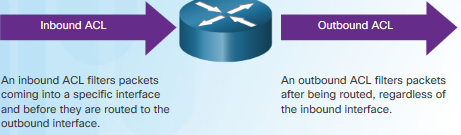
\includegraphics[scale=1]{pictures/InOut.PNG}
	\end{figure}
If the packet matches a statement, the packet is either permitted or denied. If the packet is accepted, it is then checked against routing table entries to determine the destination interface. If a routing table entry exists for the destination, the packet is then switched to the outgoing interface, otherwise the packet is dropped.\par 
Next, the router checks whether the outgoing interface has an ACL. If an ACL exists, the packet is tested against the statements in the list. If the packet matches a statement, it is either permitted or denied.\par 
If there is no ACL or the packet is permitted, the packet is encapsulated in the new Layer 2 protocol and forwarded out the interface to the next device.
\subsection{Numbered and Named ACLs}
Standard and extended ACLs can be created using either a number or a name to identify the
ACL and its list of statements.
\paragraph{Numbered ACL} Assign a number based on the following rules:
	\begin{itemize}
		\item (1 to 99) and (1300 to 1999): Standard ACL
		\item (100 to 199) and (2000 to 2699): Extended ACL
	\end{itemize}
\paragraph{Named ACL} Assign a name based on the following rules:
	\begin{itemize}
		\item Cannot contain spaces or punctuation
		\item Names are case-sensitive
		\item Can contain alphanumeric characters
		\item It is suggested that the name be written in CAPITAL LETTER
	\end{itemize}	
\section{Standard ACL}
\subsection{Overview}
A standard IPv4 ACL can filter traffic based on source IP addresses only. Unlike an extended ACL, it cannot filter traffic based on Layer 4 ports.\par 
Because standard ACLs do not specify destination addresses, place them as close to the destination as possible. If a standard ACL was placed at the source of the traffic, the "permit" or "deny" will occur based on the given source address no matter where the traffic is destined.\par 
\subsection{Standard ACL placement}
In the figure \ref{standardACLex}, the administrator wants to prevent traffic originating in the 192.168.10.0/24 network from reaching the 192.168.30.0/24 network. \par
	\begin{figure}[hbtp]
	\caption{Standard ACL placement}\label{standardACLex}
	\centering
	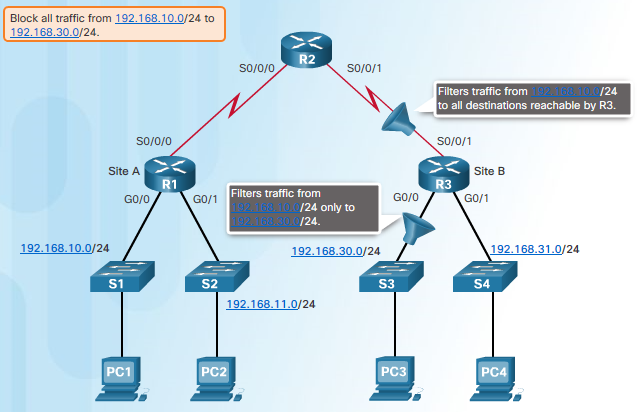
\includegraphics[ width=0.8\textwidth ]{pictures/standardACLex.PNG}
	\end{figure}
Following the basic placement guidelines of placing the standard ACL close to the destination, the figure shows two possible interfaces on R3 to apply the standard ACL:
\begin{itemize}
\item R3 S0/0/1 interface - Applying a standard ACL to prevent traffic from 192.168.10.0/24 from entering the S0/0/1 interface will prevent this traffic from reaching 192.168.30.0/24 and all other networks that are reachable by R3. This includes the 192.168.31.0/24 network. Because the intent of the ACL is to filter traffic destined only for 192.168.30.0/24, a standard ACL should not be applied to this interface.
\item R3 G0/0 interface - Applying the standard ACL to traffic exiting the G0/0 interface will filter packets from 192.168.10.0/24 to 192.168.30.0/24. This will not affect other networks that are reachable by R3. Packets from 192.168.10.0/24 will still be able to reach 192.168.31.0/24.
\end{itemize}
\section{Extended ACLs}
\subsection{Overview}
Extended ACLs filter packets based on:
	\begin{itemize}
	\item Protocol type (e.g. IP, ICMP, UDP, TCP)
	\item Source and destination IP addresses
	\item Source and destination TCP and UDP ports (HTTP port 80, SSH port 22, etc.)
	\end{itemize}
Extended ACLs are used more often than standard ACLs because they provide a greater degree of control. We usually locate extended ACLs as close as possible to the source of the traffic to be filtered. This way, undesirable traffic is denied close to the source network without crossing the network infrastructure.
\subsection{Extended ACL Placement}
In figure \ref{extendedACLex}, the administrator wants to deny Telnet and FTP traffic from the .11 network to Company B’s 192.168.30.0/24 (.30, in this example) network. At the same time, all other traffic from the .11 network must be permitted to leave Company A without restriction.\par 
	\begin{figure}[hbtp]
	\caption{Extended ACL Placement}\label{extendedACLex}
	\centering
	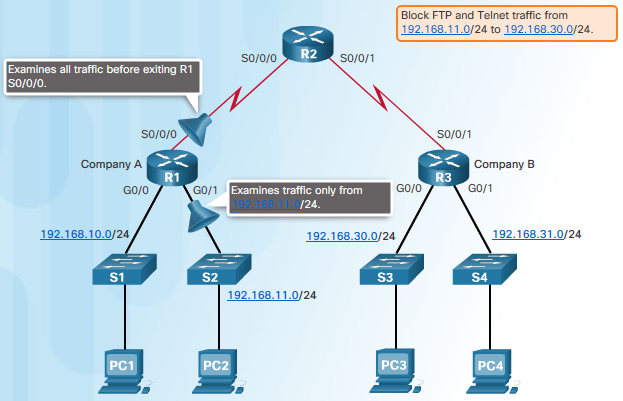
\includegraphics[ width=0.8\textwidth ]{pictures/extendedACLex.PNG}
	\end{figure}
A better solution is to place an extended ACL on R1. There are two possible interfaces on R1 to apply the extended ACL:
\begin{itemize}
\item R1 S0/0/0 interface (outbound) - One possibility is to apply an extended ACL outbound on the S0/0/0 interface. Because the extended ACL can examine both source and destination addresses, only FTP and Telnet packets from 192.168.11.0/24 will be denied. Other traffic from 192.168.11.0/24 and other networks will be forwarded by R1. The disadvantage of placing the extended ACL on this interface is that all traffic exiting S0/0/0 must be processed by the ACL including packets from 192.168.10.0/24.
\item R1 G0/1 interface (inbound) - Applying an extended ACL to traffic entering the G0/1 interface means that only packets from the 192.168.11.0/24 network are subject to ACL processing on R1. Because the filter is to be limited to only those packets leaving the 192.168.11.0/24 network, applying the extended ACL to G0/1 is the best solution.
\end{itemize}
\section{IPv6 ACLs}
In IPv4 there are two types of ACLs, standard and extended and both types of ACLs can be either numbered or named ACLs. With IPv6, there is only one type of ACL, which is equivalent to an IPv4 extended named ACL and there are no numbered ACLs in IPv6. \\
Because IPv6 ACLs must be configured with both a source and a destination, they should be applied closest to the source of the traffic. \\
An IPv4 ACL and an IPv6 ACL cannot share the same name. There are three significant differences between IPv4 and IPv6 ACLs:
	\begin{itemize}
	\item The command used to apply an IPv6 ACL to an interface is \texttt{ipv6 traffic-filter} command.
	\item IPv6 ACLs do not use wildcard masks but instead specifies the prefix-length
	\item Besides \texttt{deny ipv6 any any}, An IPv6 ACL adds two implicit permit statements at the end of each IPv6 access list: \texttt{permit icmp any any nd-na} and \texttt{permit icmp any any nd-ns}
	\end{itemize}
\section{Configurations}
\begin{example}
The figure shows an example of an ACL designed to permit a single network. Only traffic from the 192.168.10.0/24 network will be permitted out the Serial 0/0/0 interface.\\
\begin{listing}
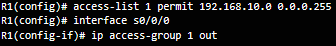
\includegraphics[scale=1]{pictures/example0.PNG} 
\end{listing}
\end{example}
\begin{example}
Figure below shows the commands used to configure a standard named ACL on router R1, interface G0/0, which denies host 192.168.11.10 access to the 192.168.10.0 network.\\
\begin{listing}
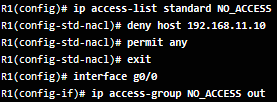
\includegraphics[scale=1]{pictures/example1.PNG} 
\end{listing}
\end{example}
\begin{example}
Design an IPv4 named access list HQServer to prevent any computers attached to the g0/0 interface of the Branch router from accessing HQServer.pka (172.16.0.1). All other traffic is permitted. Configure the access list on the appropriate router, apply it to the appropriate interface and in the appropriate direction.
	\begin{verbatim}
Branch(config)#ip access-list extended HQServer
Branch(config-ext-nacl)#deny ip any host 172.16.0.1
Branch(config-ext-nacl)#permit ip any any
Branch(config-ext-nacl)#exit
Branch(config)#int g0/0
Branch(config-if)#ip access-group HQServer in
	\end{verbatim}
\end{example}
\begin{example}
Design an IPv4 named access list BranchServer to prevent any computers attached to the Gigabit Ethernet 0/0 interface of the HQ router from accessing the HTTP and HTTPS service of the Branch server (172.16.128.1/20). All other traffic is permitted. Configure the access list on the appropriate router, apply it to the appropriate interface and in the appropriate direction.
\begin{verbatim}
HQ(config)#ip access-list extended BranchServer
HQ(config-ext-nacl)#deny tcp any host 172.16.128.1 eq 80
HQ(config-ext-nacl)#deny tcp any host 172.16.128.1 eq 443
HQ(config-ext-nacl)#permit ip any any
HQ(config-ext-nacl)#exit
HQ(config)#int g0/0
HQ(config-if)#ip access-group HQServer in
\end{verbatim}
\end{example}
\begin{example}
 Design an IPv6 access-list named NO-B1 to prevent any IPv6 traffic originating on B1 (2001:DB8:ACAD:B1::2/64) to reach the BranchServer.pka (2001:DB8:ACAD:B2::3/64). No traffic should be permitted from B1 to BranchServer.pka. Apply the IPv6 access to the most appropriated location (interface and direction).
\begin{verbatim}
Branch(config)#ipv6 access-list NO-B1
Branch(config-ipv6-acl)#deny ipv6 host 2001:DB8:ACAD:B1::2 host 2001:DB8:ACAD:B2::3
Branch(config-ipv6-acl)#permit ipv6 any any
Branch(config-ipv6-acl)#exit
Branch(config)#int g0/1
Branch(config-if)#ipv6 traffic-filter NO-B1 out
\end{verbatim}
\end{example}
\begin{example}
The network administrator configured an ACL to allow users from the 192.168.10.0/24 network to browse both insecure and secure websites. In this topology (figure \ref{example4}) the interface closest to the source of the target traffic is the G0/0 interface of R1.
	\begin{figure}[hbtp]
	\caption{Extended ACL example}\label{example4}
	\centering
	\subfigure[]{ 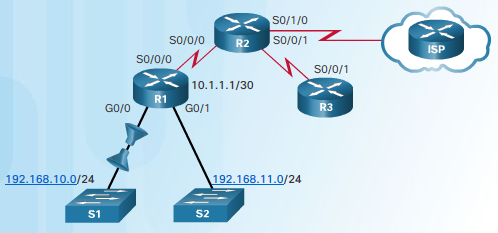
\includegraphics[ width=0.7\textwidth ]{pictures/example4-1.PNG} }
	\subfigure[]{ 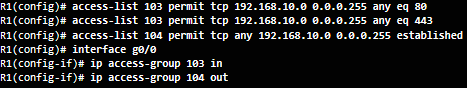
\includegraphics[ scale=1 ]{pictures/example4-2.PNG} }
	\end{figure}
Web request traffic from users on the 192.168.10.0/24 LAN is inbound to the G0/0 interface. Return traffic from established connections to users on the LAN is outbound from the G0/0 interface. The example applies the ACL to the G0/0 interface in both directions. The inbound ACL, 103, checks for the type of traffic. The outbound ACL, 104, checks for return traffic from established connections. This will restrict 192.168.10.0 Internet access to allow only website browsing.
\end{example}
\begin{example}
Configure an extended IPv4 ACL named INTOHQ such that: 
\begin{itemize}
\item Allow any hosts from the Internet to access the County DNS Svr. There should be two ACEs, one for TCP and the other UDP. Both use port 53.
\item Allow any hosts from the Internet to access the County Web Svr. Only port 80 is needed.
\item Allow return TCP traffic from the Internet that was initiated from the hosts in the Central networks to pass (with the established keyword).
\item Apply the ACL to the Central S0/0/0 interface.
\end{itemize}
\begin{verbatim}
ip access-list extended INTOHQ
	permit tcp any host 172.16.10.5 eq 53
	permit udp any host 172.16.10.5 eq 53
	permit tcp any host 172.16.10.10 eq 80
	permit tcp any any established
	exit
interface s0/0/0
	ip access-group INTOHQ IN
exit
\end{verbatim}
\end{example}
\begin{example}
Configure an extended ACL named SNMPACCESS such that 
\begin{itemize}
\item The SNMP operation runs UDP on port 161.
\item Allow only the County-Admin-PC to access the Central router for the SNMP connection.
\item SNMP connections from other hosts on the Central LAN should fail.
\item Allow all other IP traffic.
\item Apply this ACL on the Central router, G0/0 interface.
\end{itemize}
\begin{verbatim}
ip access-list extended SNMPACCESS
	permit udp host 192.168.10.5 host 192.168.10.1 eq 161
	deny udp any host 192.168.10.1 eq 161
	permit ip any any
	exit
interface g0/0
	ip access-group SNMPACCESS in
exit

\end{verbatim}
\end{example}
\section{Troubleshoot}
Using the \texttt{show access-lists} command to reveal most of the common ACL errors. The most common errors are entering ACEs in the wrong order and not applying adequate criteria to the ACL rules. Following these steps to troubleshoot ACL:
\begin{enumerate}
\item Check the criteria of ACL rules
\item Check the order of ACEs
\item Check the direction of ACL (inbound, outbound)
\item Check the location of ACL (which router, which interface). Remember that extended ACLs are placed as close as possible to the source and standard ACLs are placed as close as possible to the destination.
\end{enumerate}
\begin{example}
The 192.168.10.0/24 network cannot use TFTP to connect to the 192.168.30.0/24 network.\\
\begin{listing}
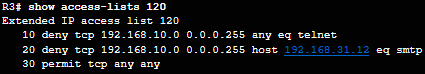
\includegraphics[scale=1]{pictures/example2.PNG} 
\end{listing}\\
Solution: The 192.168.10.0/24 network cannot use TFTP to connect to the 192.168.30.0/24 network because TFTP uses the transport protocol UDP. Statement 30 in access list 120 allows all other TCP traffic. However, because TFTP uses UDP instead of TCP, it is implicitly denied. Recall that the implied deny any statement does not appear in show access-lists output and therefore matches are not shown. Statement 30 should be \texttt{permit ip any any}.
\end{example}
\begin{example}
The 192.168.11.0/24 network can use Telnet to connect to 192.168.30.0/24, but according to company policy, this connection should not be allowed. The results of the show access-lists 130 command indicate that the permit statement has been matched.\\
\begin{listing}
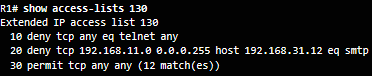
\includegraphics[scale=1]{pictures/example3.PNG} 
\end{listing}\\
The 192.168.11.0/24 network can use Telnet to connect to the 192.168.30.0/24 network because the Telnet port number in statement 10 of access list 130 is listed in the wrong position in the ACL statement. Statement 10 currently denies any source packet with a port number that is equal to Telnet. To deny Telnet traffic inbound on G0/1, deny the destination port number that is equal to Telnet, for example, 10 deny tcp 192.168.11.0 0.0.0.255 192.168.30.0 0.0.0.255 eq telnet.
\end{example}